\documentclass[border=10pt]{standalone}
\usepackage{tikz}
\usepackage{amsmath}
\usetikzlibrary{positioning, shapes.geometric, arrows.meta, fit, backgrounds, calc}

\begin{document}
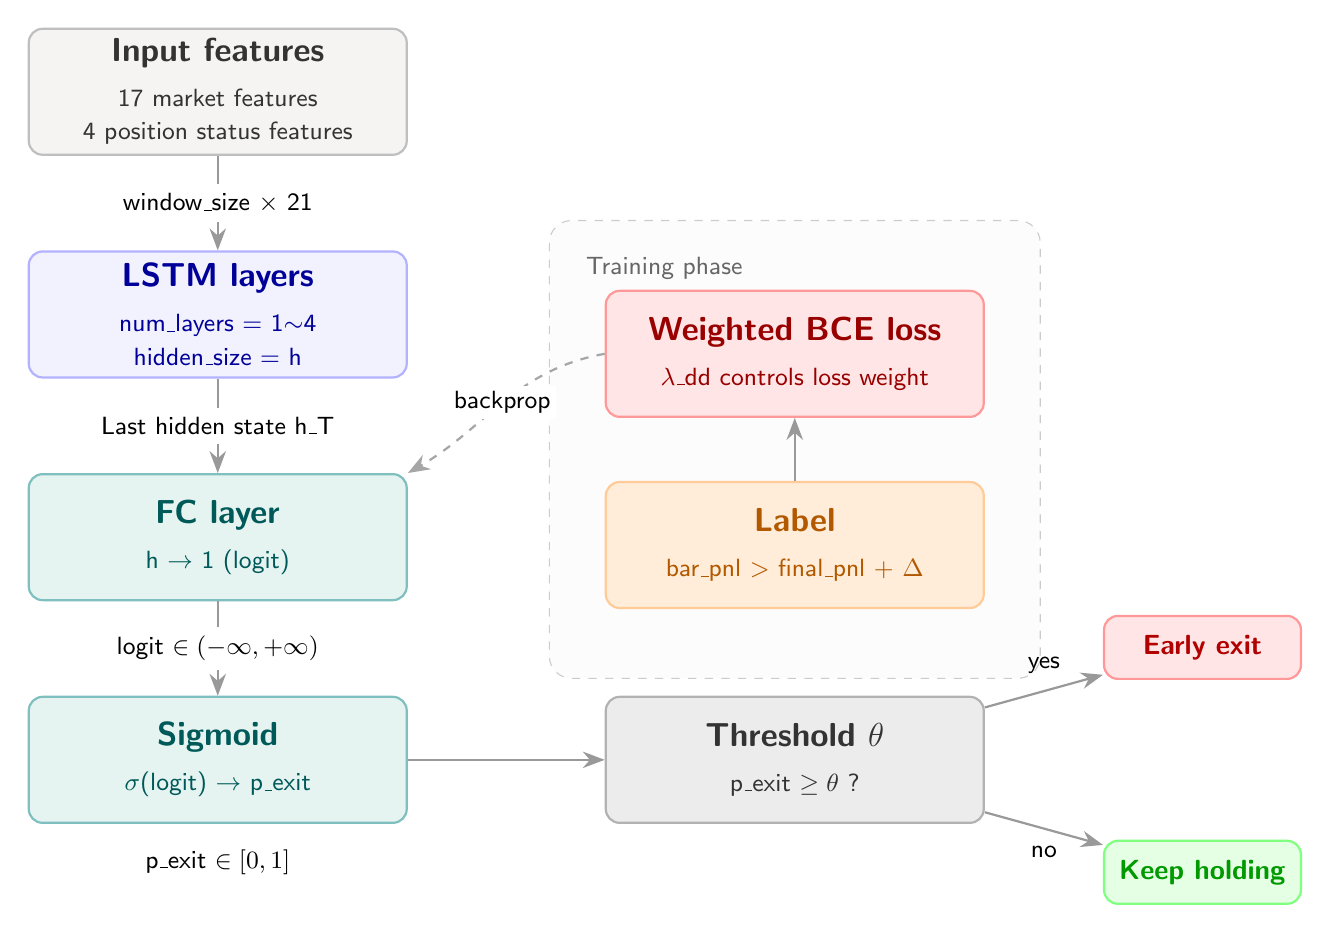
\begin{tikzpicture}[
    node distance=1.2cm and 2.5cm,
    box/.style={rectangle, rounded corners=5pt, minimum width=4.8cm, minimum height=1.6cm, align=center, draw, thick, font=\sffamily},
    input/.style={box, fill=yellow!5!gray!10, draw=gray!50, text=black!80},
    lstm/.style={box, fill=blue!5, draw=blue!30, text=blue!60!black},
    fc/.style={box, fill=green!10!teal!10, draw=teal!50, text=teal!70!black},
    sig/.style={box, fill=green!10!teal!10, draw=teal!50, text=teal!70!black},
    thresh/.style={box, fill=gray!15, draw=gray!60, text=black!80},
    loss/.style={box, fill=red!10, draw=red!40, text=red!60!black},
    lbl/.style={box, fill=orange!15, draw=orange!40, text=orange!70!black},
    outyes/.style={box, minimum width=2.5cm, minimum height=0.8cm, fill=red!10, draw=red!40, text=red!70!black},
    outno/.style={box, minimum width=2.5cm, minimum height=0.8cm, fill=green!10, draw=green!50, text=green!60!black},
    arr/.style={-{Stealth[scale=1.2]}, thick, draw=gray!80},
    dasharr/.style={-{Stealth[scale=1.2]}, dashed, thick, draw=gray!70}
]

\node[input] (in) {\textbf{\large Input features}\\[1.5mm] \small 17 market features \\ \small 4 position status features};

\node[lstm, below=of in] (lstm) {\textbf{\large LSTM layers}\\[1.5mm] \small num\_layers = 1$\sim$4 \\ \small hidden\_size = h};

\node[fc, below=of lstm] (fc) {\textbf{\large FC layer}\\[1.5mm] \small h $\rightarrow$ 1 (logit)};

\node[sig, below=of fc] (sig) {\textbf{\large Sigmoid}\\[1.5mm] \small $\sigma$(logit) $\rightarrow$ p\_exit};

\draw[arr] (in) -- (lstm) node[midway, fill=white, font=\small\sffamily] {window\_size $\times$ 21};
\draw[arr] (lstm) -- (fc) node[midway, fill=white, font=\small\sffamily] {Last hidden state h\_T};
\draw[arr] (fc) -- (sig) node[midway, fill=white, font=\small\sffamily] {logit $\in (-\infty, +\infty)$};

\node[below=0.2cm of sig, font=\small\sffamily] {p\_exit $\in [0, 1]$};

\node[thresh, right=2.5cm of sig] (thresh) {\textbf{\large Threshold $\theta$}\\[1.5mm] \small p\_exit $\geq \theta$ ?};
\draw[arr] (sig) -- (thresh);

\node[outyes, above right=0.2cm and 1.5cm of thresh] (yes) {\textbf{Early exit}};
\node[outno, below right=0.2cm and 1.5cm of thresh] (no) {\textbf{Keep holding}};

\draw[arr] (thresh) -- (yes) node[midway, above=1mm, font=\small\sffamily] {yes};
\draw[arr] (thresh) -- (no) node[midway, below=1mm, font=\small\sffamily] {no};

\node[loss, right=2.5cm of lstm, yshift=-0.5cm] (loss) {\textbf{\large Weighted BCE loss}\\[1.5mm] \small $\lambda$\_dd controls loss weight};
\node[lbl, below=0.8cm of loss] (label) {\textbf{\large Label}\\[1.5mm] \small bar\_pnl $>$ final\_pnl + $\Delta$};

\draw[arr] (label) -- (loss);

\begin{scope}[on background layer]
    \node[rectangle, rounded corners=8pt, dashed, draw=gray!40, fill=gray!2, inner xsep=20pt, inner ysep=25pt, fit=(loss) (label)] (trainbox) {};
    \node[anchor=north west, font=\small\sffamily, text=gray!80!black] at ([xshift=10pt, yshift=-10pt]trainbox.north west) {Training phase};
\end{scope}

\draw[dasharr] (loss.west) to[out=190, in=30] node[midway, fill=white, font=\small\sffamily, inner sep=2pt] {backprop} (fc.north east);

\end{tikzpicture}
\end{document}